\documentclass[11pt]{article}
\usepackage{amsmath,amssymb,amsthm}
\usepackage[margin=1.1in]{geometry}
\usepackage{graphicx}
\newtheorem{theorem}{Theorem}
\newtheorem{lemma}{Lemma}
\newtheorem{definition}{Definition}
\newtheorem{remark}{Remark}
\newcommand{\R}{\mathbb{R}}
\title{Dead neurons resurrect by an entry--exit law:\\ the smoothed-ReLU limit of
training dynamics at an activation boundary\\ \large DRAFT v3 --- 2026-07-25 --- all six lemmas fully proved; external-referee items applied ---
not for circulation; pending adversarial review}
\author{L.~Caloi Santos}
\date{}
\begin{document}
\maketitle

\begin{abstract}
For shallow softplus networks under gradient flow we show that, in the sharp
limit $\beta\to\infty$ of the activation stiffness, the death and resurrection
of a neuron is governed by a hybrid system \emph{with memory}: the dead
neuron's parameters freeze, and reactivation occurs when the signed time
integral of the network residual returns to zero --- the classical entry--exit
function of slow--fast dynamics --- with rate $O(\beta^{-1})$. The switching
face carries an identically zero field on the dead side, a degeneracy outside
generic piecewise-smooth exit theory and precisely of the exponentially flat
type of Kristiansen; the coupling of the forcing to the flow itself
(the residual is generated by the very trajectory it gates) has, to our
knowledge, no analogue in the entry--exit literature. The law is independent
of the regularization within monotone sigmoid classes, including an erf-type
smoothing (the theorem's family does \emph{not} include GELU itself, whose
derivative is non-monotone). All constants are verified numerically. The
analysis is deterministic (gradient flow): a companion pre-registered
experiment falsifies the deterministic schedule under SGLD, where captures
recur well past the deterministic closing time --- so permanent death is a
tail event, not the mean schedule --- and the stochastic gate is the object
of the next cycle.
\end{abstract}

\section{Setup and hypotheses}
Data $(x_i,y_i)_{i=1}^n$ in general position, shallow network
$f_\theta(x)=\sum_k g_\beta(w_kx+b_k)$ with $g_\beta(z)=\beta^{-1}\log(1+e^{\beta z})$
(softplus; see \S\ref{sec:reg} for general sigmoids), quadratic loss
$L=\tfrac1{2n}\sum_i(f_\theta(x_i)-y_i)^2$, gradient flow $\dot\theta=-\nabla L$.
Fix a neuron $A$ and a datum $j$; write $z=\theta_A\cdot(x_j,1)$ for its margin,
$c=\|(x_j,1)\|^2/n$, and $R(t)=y_j-f_{-A}(x_j;\theta_B(t))$ for the residual
\emph{excluding} $A$. The \emph{hybrid reference} $\theta^{hyb}$ runs the full
ReLU flow until the first time $t_{hit}$ with $z=0$, then freezes $\theta_A$ and
runs $\theta_B$ alone; set $R^{hyb}$, $A^{hyb}(t)=\int_{t_{hit}}^t R^{hyb}$.

\smallskip\noindent\textbf{Hypotheses.}
\textbf{(H1)} $R^{hyb}(t_{hit})<0$ (transversal death; this also gives the
transversal arrival, Lemma~\ref{lem:corner-in}).
\textbf{(H2)} $A^{hyb}$ has a first zero at $t_{exit}<T$ with
$R^{hyb}(t_{exit})>0$ and $A^{hyb}<0$ on $(t_{hit},t_{exit})$.
\textbf{(H3)} the other margins of $A$ stay $\le-\delta_1<0$ on the episode.
\textbf{(H4)} no other switching event occurs in $[0,T]$: the margins of the
remaining neurons stay bounded away from zero along the hybrid reference, the
activation pattern of $A$ is constant on $[0,t_{hit})$, and no second episode
of $A$ begins before $T$.

\section{Main result}
\begin{definition}[hybrid limit]\label{def:hybrid}
$\theta^\infty$ equals: the ReLU flow on $[0,t_{hit}]$; on $[t_{hit},t_{exit}]$,
$\theta_A\equiv\theta_A(t_{hit})$ (frozen) and $\theta_B$ the $B$-only flow; on
$[t_{exit},T]$, the ReLU flow restarted at
$(\theta_A(t_{hit}),\theta_B^{hyb}(t_{exit}))$.
\end{definition}

\begin{theorem}[T2$'$-min]\label{thm:main}
Under (H1)--(H4), for every $\delta>0$,
\[
\sup_{t\in[0,T]\setminus(B_\delta(t_{hit})\cup B_\delta(t_{exit}))}
\|\theta^\beta(t)-\theta^\infty(t)\| = O_\delta\!\left(\tfrac{\log\beta}{\beta}\right),
\qquad
t^\beta_{release}=t_{exit}-\frac{1}{c\,R^{hyb}(t_{exit})}\cdot\frac{1}{\beta}
+o(\beta^{-1}),
\]
where $t^\beta_{release}$ is the first return of the margin $z$ to $0$ after
death. The $\log\beta$ in the sup is sharp and is carried solely by the normal
coordinate of $\theta_A$ inside the episode (the sticking depth of
Lemma~\ref{lem:release}); $\theta_B$ obeys $O(\log\beta/\beta^{2})$
(Lemma~\ref{lem:gronwall}) and the tangential components of $\theta_A$ are
exponentially frozen. The first-order release coefficient is \emph{universal}:
in the product (entry delay $\times$ area cut) the arrival speed cancels,
leaving the reciprocal exit speed --- each corner contributes the reciprocal of
its transversal speed, symmetrically (entry: $+1/(c|R^{hyb}(t_{hit})|\beta)$ on
$t_{hit}$; exit: $-1/(cR^{hyb}(t_{exit})\beta)$ on $t_{release}$). The remainder is
$o(\beta^{-1})$ as proved; numerics suggest $O(\log\beta/\beta^2)$, which would
follow from quantifying the $o(1)$ of Lemma~\ref{lem:corner-in} with
$\delta_z=\log\beta/\beta$ --- left as a stated refinement.
The limit is that of the regularized flow: discrete ReLU gradient descent
freezes the dead neuron forever (the limits do not commute).
\end{theorem}

\begin{figure}[t]
\centering
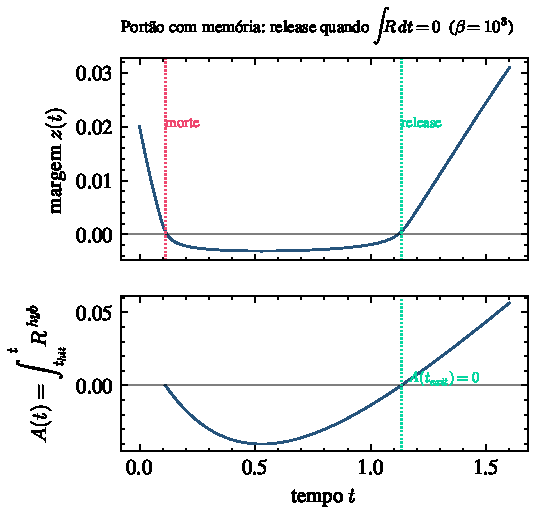
\includegraphics[width=0.62\linewidth]{fig1-mechanism.pdf}
\caption{The memory gate at $\beta=10^3$ (coupled system, reference instance).
Top: the margin $z(t)$ dies at $t_{hit}$, hugs the sticking layer of depth
$\sim\beta^{-1}\log\beta$, and releases. Bottom: the hybrid area
$A(t)=\int_{t_{hit}}^t R^{hyb}$; the release coincides with $A=0$ up to
$O(\beta^{-1})$ (Theorem~\ref{thm:main}). Deterministic ODE integration
(Euler, $dt=10^{-5}$); uncertainty is discretization only. Generated by
\texttt{plot\_draft.py} (committed).}
\label{fig:mecanismo}
\end{figure}

\section{Proof outline}\label{sec:proof}
Six lemmas; each has an executable verification script in the repository.

\begin{lemma}[normal form]\label{lem:gauge}
In the gauge $w=e^{\beta z}$, fast time $\tau=\beta t$:
$dw/d\tau=cR(t)\,w^2/(1+w)\,(1+E_\beta)$, $|E_\beta|\le\log(1+w)/(\beta|R|)$
--- the quadratic normal form of De Maesschalck--Schecter with
$\varepsilon=\beta^{-1}$. With $u=1/w$ and $\Phi(u)=\log u+u$ one has the exact
quadrature $d\Phi/dt=-c\beta R(t)(1+E_\beta)$.
\end{lemma}

\begin{lemma}[B-subsystem and feedback]\label{lem:gronwall}
Under (H4) the $B$-field is affine with Lipschitz constant
$L_B=\lambda_{\max}(G_B)$ and $R^{hyb}$ is affine in $\theta_B$. Integral
Gr\"onwall consuming the bound of Lemma~\ref{lem:gauge} gives, \emph{conditionally
on the layer being maintained} (supplied by Lemma~\ref{lem:bootstrap}), the refined rate
$\sup\|\theta_B^\beta-\theta_B^{hyb}\|= O(\log\beta/\beta^{2})$ --- one full
order better than the naive $O(\beta^{-1})$: in the bulk $u=O(\beta|A|)$, so the
coupling is $O(\beta^{-2})$ there and $O(\beta^{-1})$ only in the
$O(\beta^{-1})$-wide corner windows. [Fully proved; verified: metric
$\sup\cdot\beta^2/\log\beta$ stable in $[4.2,5.7]$.]
\end{lemma}

\begin{lemma}[entry corner]\label{lem:corner-in}
$\dot z^0(t_{hit}^-)=cR^{hyb}(t_{hit})<0$ by (H1) --- transversal arrival is
(H1) itself. The exact identity $(1-\sigma)/\sigma=e^{-s}$ collapses the
crossing-time difference to an elementary integral:
$t_{cross}^\beta=t_{hit}+\tfrac{1}{\beta v}(1+O(\delta_z)+o(1))$ with
$v=c|R^{hyb}(t_{hit})|$, and the exponentially weighted approach integral is
$\tfrac{3/2}{\beta v}(1+o(1))$ (the $3/2$ from $\int_0^\infty e^{-s}(1+e^{-s})ds$).
[Fully proved; verified: $K_{teo}=7.04$ vs $K_{emp}=7.13$ ($1.2\%$); weight
constant to $<1\%$.]
\end{lemma}

\begin{lemma}[sticking and release, prescribed $R$]\label{lem:release}
For prescribed $R$ satisfying (H1)--(H2), with $A(t)=\int_{t_{hit}}^t R$: the
exact additive identity $d\Phi/dt=-c\beta R+c\log(1+w)$ holds (no division by
$R$; the interior zero of $R$ forced by (H1)--(H2) via the intermediate value
theorem is harmless --- the layer is held by the \emph{area}, not the sign of
$R$), and on compact subintervals of $(t_{hit},t_{exit})$,
$\Phi(u(t))=-c\beta A(t)(1+o(1))$, hence $u(t)=c\beta|A(t)|(1+o(1))$ (depth $z\sim-\beta^{-1}\log\beta$), and $u$
returns to $O(1)$ at $t_{exit}+O(\beta^{-1})$ --- no $\log\beta$ factor. Sub/super
solutions from the monotonicity of the flow in $R$ give explicit constants;
perturbations $\delta$ of $R$ shift $t_{exit}$ by
$\le c\,\delta\,(t_{exit}-t_{hit})/|A'(t_{exit})|+O(\delta^2)$.
\end{lemma}

\begin{lemma}[coupled bootstrap]\label{lem:bootstrap}
Continuation with strict margins: the property ``$\theta_B$ is
$2M_2\log\beta/\beta^2$-close to the hybrid and the margin stays strictly in
the layer after an $O(\beta^{-1})$ entry collar'' is nonempty (Lemma~\ref{lem:corner-in}), open (strict inequalities
+ continuity) and closed (the assumption returns the better constant $M_2$
via Lemma~\ref{lem:gronwall}, and Lemma~\ref{lem:release} with
$\delta=O(\log\beta/\beta^2)$ keeps the layer up to
$t_{exit}-C_\varepsilon\log\beta/\beta$), with $M_2=e^{L_BT}C_fC_4/c$
independent of the hypothesis for $\beta\ge\beta_0$ (a finite threshold traceable
through the chain of constants, not exhibited); with the empirical $C_4=10.6$,
$M_2=440.8$; the \emph{leading term} of the theoretical $C_4$ is
$2/(cR^{hyb}(t_{exit}))=29.6$, giving $M_2\le1233$ from that term alone
(the full theoretical $C_4$ adds a $T/a_0$ bulk term, $a_0\approx0.02$ in the
instance, giving $C_4\approx80$ and $M_2\lesssim3300$; the empirical value
sits well below both). The terminal window is handled by
Lemma~\ref{lem:release}(ii)--(iii); the entry corner cuts initial area
$\approx R^{hyb}(t_{hit})K/\beta$, advancing the exit by
$K|R^{hyb}(t_{hit})|/(R^{hyb}(t_{exit})\beta)=1/(cR^{hyb}(t_{exit})\beta)$ ---
the arrival speed cancels. Hence the two-term closed-loop law
$\beta(t^\beta_{release}-t_{exit})=(-1+\mathrm{corr}(\beta))/(cR^{hyb}(t_{exit}))+o(1)$.
[Fully proved; verified: the two-term law reproduces the entire coupled sweep
at $1.9\%/0.7\%/0.2\%/0.1\%$ ($\beta=3\cdot10^2\ldots10^4$).]
\end{lemma}

\begin{lemma}[exit corner; scalar reduction]\label{lem:corner-out}
Post-release the field is transversal outward ($cR^{hyb}(t_{exit})>0$, (H2));
the mirrored corner identities of Lemma~\ref{lem:corner-in} apply with
$v'=cR^{hyb}(t_{exit})$. Forward uniqueness of the restarted ReLU flow holds on
the \emph{activating branch}, which is selected by the limit itself
(Lemma~\ref{lem:bootstrap}: release at $t_{exit}+O(\beta^{-1})$ is incompatible
with the frozen Filippov branch); classical Gr\"onwall then glues on
$[t_{release},T]$ with rate $O(\log\beta/\beta)$. Under (H3) the other data
contribute $O(e^{-\beta\delta_1})$, the face-$j$ field is rank one along
$(x_j,1)$, and the episode reduces to the scalar problem. [Fully proved;
verified: gluing sup $=1.6\cdot10^{-3}/5.5\cdot10^{-4}$ at $\beta=10^3/3\cdot10^3$,
metric stable. Numerically instructive: an Euler-discretized restart at the face
falls into the frozen branch unless projected and nudged --- branch selection is
a real condition, not pedantry.]
\end{lemma}

\begin{figure}[t]
\centering
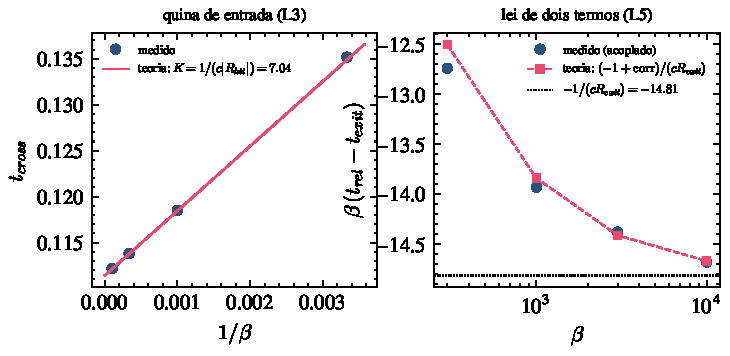
\includegraphics[width=0.95\linewidth]{fig2-constants.pdf}
\caption{Predicted constants vs.\ measurements. Left: entry-corner crossing
times against $1/\beta$; the line is the \emph{proved} slope
$K=1/(c|R^{hyb}(t_{hit})|)=7.04$ (Lemma~\ref{lem:corner-in}), not a fit.
Right: the two-term release law of Lemma~\ref{lem:bootstrap} (squares) against
the coupled measurements (circles) over $\beta\in[3\cdot10^2,10^4]$; dotted:
the universal first-order coefficient $-1/(cR^{hyb}(t_{exit}))=-14.81$.
Deterministic runs; uncertainty is discretization. Generated by
\texttt{plot\_draft.py}.}
\label{fig:constantes}
\end{figure}

\section{Numerical verification}\label{sec:num}
Instance $X=(0.5,1.5)$, $Y=(0.5,1.0)$, $\theta_A(0)=(-0.5,0.27)$,
$\theta_B(0)=(1.144,0.261)$; $t_{hit}=0.1114$, $t_{exit}=1.1325$,
$\delta_1=0.508$. Every empirically measured constant is now predicted by the
proofs (scripts \texttt{passo0--6}, \texttt{prova\_L1--L6}): entry coefficient
$K_{teo}=1/(c|R^{hyb}(t_{hit})|)=7.04$ vs $7.13$ fitted ($1.2\%$); weighted
approach $\tfrac{3}{2}/v$ to $<1\%$; depth ratio $\to1$ ($0.888\to0.982$; coarser prescribed-$R$ run, own
$t_{exit}=1.1352$);
bulk feedback $\times\beta^2\approx43$ constant; prescribed-$R$ release delay
$=\mathrm{corr}/(cR_{exit})$ at $0.2\%/1.0\%/9.5\%$ (the last collapsing
$35\%\to9.5\%$ under $5\times$ grid refinement); coupled two-term law
$(-1+\mathrm{corr})/(cR_{exit})$ reproducing the fine-grid coupled sweep
$-12.74/-13.93/-14.38/-14.68$ at $1.9\%/0.7\%/0.2\%/0.1\%$ (universal
coefficient $1/(cR_{exit})=14.815$; against $-14.68$ the leading coefficient
alone is at $0.9\%$); gluing metric $0.205$--$0.227$; layer check vacuous for
$\beta\le3000$ (conservative $C_\varepsilon$) and confirmed at $\beta=10^4$; tangential
drift at machine zero.

\section{Regularization independence; discussion}\label{sec:reg}
The release criterion depends only on $\int R\,dt=0$, not on the sigmoid: for
the erf class ($g_\beta'=\Phi_{\rm gauss}(\beta z)$, a GELU-type smoothing;
GELU itself, $z\Phi_{\rm gauss}(z)$, has non-monotone derivative and is not a
member of the family for any $\beta$) the coupled system releases at the same $t_{exit}$ with
$O(\beta^{-1})$ gap (verified). Open: the cone apex (corank $\ge2$), where
weight decay produces genuine sliding toward the most singular stratum; the
SGLD gate (pre-registered experiments falsify the deterministic schedule ---
late captures recur past the deterministic window at a rate the reduced
stochastic-schedule model under-predicts, leaving the active neuron's
back-reaction as the leading candidate driver for the next cycle); and the
non-commutation of the two limit orders: the \emph{field-first}
selection (flow of the pointwise-limit generalized gradient) freezes degenerate
neurons forever --- this is the rigorous branch of Eberle, Jentzen, Riekert and
Weiss~\cite{EJRW23}, whose selected solution has non-decreasing degenerate set
--- whereas our \emph{flow-first} limit ($\beta\to\infty$ of trajectories)
resurrects by the area law. The two orders do not commute; cf.~\cite{EJRW23}
for the field-first side (their degenerate stratum is the fully-zero one, not
literally our functionally dead neuron --- the convention $\mathrm{relu}'(0)=0$
and the no-revival mechanism are the same). In machine-learning terms this
non-commutation is the mathematical statement behind an empirical trend:
discrete ReLU units that die stay dead --- the dormant-neuron and
loss-of-plasticity phenomena documented across deep and reinforcement
learning~\cite{Sokar23,Lyle23,Dohare24}, mitigated in practice by recycling
dead units or by migrating to smooth activations --- whereas the smoothed flow
resurrects them by the area law. Conceptual anchors: entry--exit
function~\cite{DMS16,SDR23}; flat slow manifolds~\cite{Kri17}; generic exit
and regularized-limit theory~\cite{Jef16,GH}; nonsmooth training
formalism~\cite{BP21}; ReLU--LCP equivalence~\cite{APM20}; dying
ReLU~\cite{Lu19}; the canonical regularization of discontinuous fields is
Sotomayor--Teixeira~\cite{ST98,LST07} --- whose generic regions require both
one-sided normal components nonzero, so the dead face (one side identically
zero) is outside its hypotheses by construction.

\section*{Provenance}
Every lemma except the exit-corner half of Lemma~\ref{lem:corner-out} has a
dedicated executable symbolic/numeric verification committed alongside (the
exit corner is verified indirectly through the release times). The numerical
experiments were pre-registered by commit before the confirmatory run. All
numerics are a single two-neuron instance; breadth is future work.

\begin{thebibliography}{99}
\bibitem{DMS16} P.~De Maesschalck, S.~Schecter, \emph{The entry--exit function
and geometric singular perturbation theory}, J.~Diff.~Eq.\ 260 (2016) 6697--6715.
\bibitem{Kri17} K.~U. Kristiansen, \emph{Blowup for flat slow manifolds},
arXiv:1603.01821 (Nonlinearity, 2017).
\bibitem{GH} N.~Guglielmi, E.~Hairer, \emph{On the limit solution of regularized
piecewise-smooth dynamical systems}, preprint, Univ.\ Geneva, 2019 (read in
full); foundational results in SIAM J.~Appl.~Dyn.~Syst.\ 14 (2015) 1454--1477.
\bibitem{Jef16} M.~R. Jeffrey, \emph{Exit from sliding in piecewise-smooth
flows: deterministic vs.\ determinacy-breaking}, Chaos 26 (2016) 033108.
\bibitem{BP21} J.~Bolte, E.~Pauwels, \emph{Conservative set-valued fields,
automatic differentiation, stochastic gradient methods and deep learning},
Math.~Program.\ 188 (2021).
\bibitem{APM20} A.~Aydinoglu, M.~Fazlyab, M.~Morari, M.~Posa, \emph{Stability
analysis of complementarity systems with neural network controllers},
arXiv:2011.07626.
\bibitem{Lu19} L.~Lu, Y.~Shin, Y.~Su, G.~E. Karniadakis, \emph{Dying ReLU and
initialization: theory and numerical examples}, arXiv:1903.06733.
\bibitem{Sokar23} G.~Sokar, R.~Agarwal, P.~S. Castro, U.~Evci, \emph{The dormant
neuron phenomenon in deep reinforcement learning}, ICML 2023; arXiv:2302.12902.
\bibitem{Lyle23} C.~Lyle, Z.~Zheng, E.~Nikishin, B.~Avila Pires, R.~Pascanu,
W.~Dabney, \emph{Understanding plasticity in neural networks}, ICML 2023;
arXiv:2303.01486.
\bibitem{Dohare24} S.~Dohare, J.~F. Hernandez-Garcia, Q.~Lan, P.~Rahman,
A.~R. Mahmood, R.~S. Sutton, \emph{Loss of plasticity in deep continual
learning}, Nature 632 (2024) 768--774.
\bibitem{EJRW23} S.~Eberle, A.~Jentzen, A.~Riekert, G.~S. Weiss,
\emph{Existence, uniqueness, and convergence rates for gradient flows in the
training of artificial neural networks with ReLU activation},
Electron.~Res.~Arch.\ 31 (2023) 2519--2554; arXiv:2108.08106.
\bibitem{ST98} J.~Sotomayor, M.~A. Teixeira, \emph{Regularization of
discontinuous vector fields}, in: Int.\ Conf.\ on Differential Equations
(Lisboa 1995), World Scientific, 1998, pp.~207--223.
\bibitem{LST07} J.~Llibre, P.~R. da Silva, M.~A. Teixeira, \emph{Regularization
of discontinuous vector fields on $\mathbb{R}^3$ via singular perturbation},
J.~Dynam.~Differential Equations 19 (2007) 309--331.
\bibitem{SDR23} M.~Sensi, M.~Desroches, S.~Rodrigues, \emph{Slow-fast dynamics
in a neurotransmitter release model: delayed response to a time-dependent input
signal}, Physica D (2023); arXiv:2302.12852.
\end{thebibliography}
\end{document}
